\chapter{Background}
% Created 04-03-2016
% Updated 17-11-2016 Came up with proper sections and everything I wanted to say in this chapter. Started writing the first sections.
% Updated 18-11-2016 Added Research focus, MAV Design and decided not to do the Mars 2020 landing site.
% Updated 19-11-2016 Included section on reference systems.
% Updated 27-11-2016 Continued work on reference systems.
% Updated 05-02-2017 Implemented feedback

\label{ch:problembackground}
One of the current focal points of \ac{JPL} is Mars and the exploration of the Martian system \footnote{All past, current, future and proposed \ac{JPL} missions: \url{http://www.jpl.nasa.gov/missions/} [Accessed 17 November 2016]}. There are currently two planned missions to Mars: InSight and Mars 2020. 

InSight is a mission similar to the Viking and the Phoenix missions, and primarily based on the last one. It includes a lander that will perform experiments on the surface of Mars at a fixed location. Mars 2020 includes the next Mars rover and is based on the Curiosity rover. It has a similar design, but will carry different scientific instruments and will focus more on finding life on Mars. Mars 2020 is part of a larger \ac{JPL} effort to eventually return samples from the Martian surface back to Earth. This mission concept has been on the drawing board for several years now, but finally seems to be getting closer to approval. 

This sample return mission, or \ac{MSR}, will consist of three different systems and is spread out over three different missions as shown by the proposed mission architecture in \Cref{fig:proposedMSRmissionArchitecture_vaughan2016technology}. Mars 2020 is the first step (denoted by 1 in the figure) in this plan where the rover will collect samples from the surface of Mars. These samples will then be put into containment tubes and dropped on the surface of Mars. A second mission will then carry a system that will collect these samples from the surface and deliver them into a Martian orbit (see number 3 in the figure) \citep{shotwell2016drivers}. Then a third mission, currently proposed as the Mars 2022 orbiter (see number 2 in the figure), will collect the sample containment sphere in orbit and eventually deliver it back to Earth \citep{woolley2011mars}. 

Because of the potential of the \ac{MSR} mission concept and the amount of research that still has to be done on this subject, the focus was put on this \ac{JPL} effort when looking at research subjects.


\begin{figure}[H]
\centering
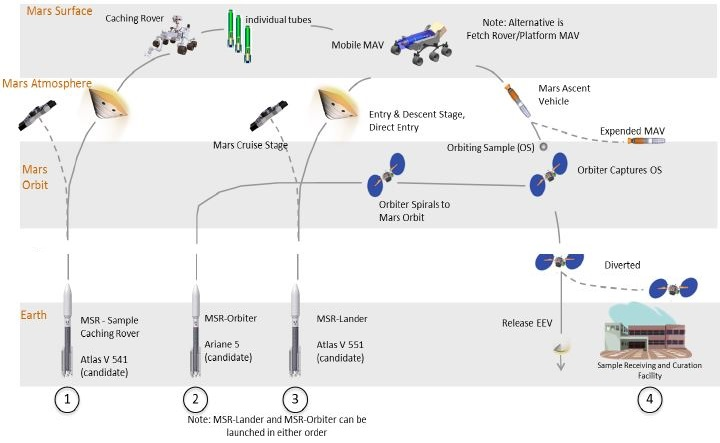
\includegraphics[width=0.79 \textwidth]{figures/heritage/proposedMSRmissionArchitecture_vaughan2016technology.jpg}
\caption{Proposed \ac{MSR} campaign architecture \citep{vaughan2016technology}.}
\label{fig:proposedMSRmissionArchitecture_vaughan2016technology}
\end{figure}



% This will serve as a general introduction to the problem
%JPL
%JPL missions
%Interesting missions

\section{Chosen Mission}
\label{sec:chosenMission}
Mars 2020 is an approved mission that is currently in the design phase, and Mars 2022 is a proposed mission that will have to be built to enhance the current communication capabilities between Mars and Earth, which is its primary objective. Therefore it is almost certain that these two missions will fly and it should be noted that for both these missions, \ac{MSR} is a secondary objective. However, this does not guarantee that the entire \ac{MSR} endeavour will be realised. This is because there is no official approval yet for the second system that will actually bring the samples from the surface back to Earth. However, this does not mean that no research is being done on the return system. 

Many designs have been envisioned over the past few years and even now engineers cannot decide on the best design. \cite{shotwell2016drivers} shows two of the proposed designs that are currently being considered. One design involves a mobile launch system based on the Curiosity rover, which will fetch the samples and then directly put them into the spherical container, as depicted in \Cref{subfig:launch_rover_shotwell2016drivers}. Once this container is filled, the sphere will be placed on top of the \ac{MAV}, which the rover will be carrying on its back, and launched into Mars orbit. The second design (\Cref{subfig:fetch_rover_shotwell2016drivers}) uses two systems: one fetch rover that will grab the samples and return them to the lander, and the lander containing the \ac{MAV}. Once the rover returns with all the samples, the sample sphere will be put on top of the \ac{MAV} and launched into orbit. There are advantages and disadvantages to both of these systems and more research is being done to determine the best option. What both of these systems have in common though, is that they have to launch the sample sphere into orbit using an \ac{MAV}. An ascent on another celestial body with an atmosphere has never been attempted before, which makes it a crucial part of the \ac{MSR} campaign. This is also why in the past several years, many researchers have looked at the \ac{MAV} ascent trajectory problem. 

\begin{figure}[H]
\centering
\subfloat[]{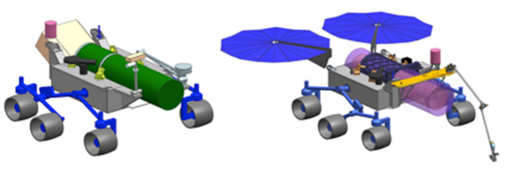
\includegraphics[width=3.1in]{figures/heritage/launch_rover_shotwell2016drivers.png}\label{subfig:launch_rover_shotwell2016drivers}}
\subfloat[]{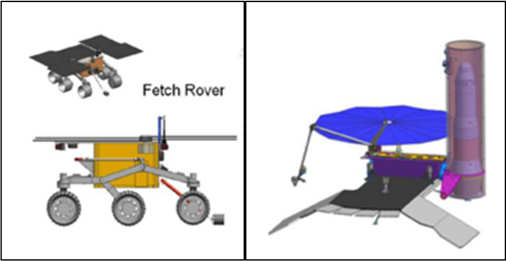
\includegraphics[width=3.1in]{figures/heritage/fetch_rover_shotwell2016drivers.png}\label{subfig:fetch_rover_shotwell2016drivers}} 
\caption{Two of the proposed concepts for the retrieval of the samples   \protect\subref{subfig:launch_rover_shotwell2016drivers} a rover carrying the \ac{MAV} powered by a radioisotope thermoelectric generator (left) or solar panels (right), \protect\subref{subfig:fetch_rover_shotwell2016drivers} a separate lander and fetch rover \citep{shotwell2016drivers} } 
\label{fig:launch_rover_shotwell2016drivers} 
\end{figure} 

%Mars Sample Return
%Focus on Ascent
%Initial conditions modelled on Mars 2020 candidate landing site (maybe leave this out...)

\section{Previous Mars Ascent Research}
\label{sec:previousMarsAscentResearch}
Not only \ac{JPL}, but also many other institutions around the world are working on the Mars ascent problem, for instance the \ac{DLR}. A selection of reference research is provided in \Cref{tab:referenceResearch}. The papers of 2015 and 2016 are based on currently ongoing research and thus represent intermediate findings.

\begin{table}[H]
\begin{center}
\caption{Previous and current Mars ascent trajectory research.}
\label{tab:referenceResearch}
\begin{tabularx}{1.0\textwidth}{|X|X|X|}
\hline 
\textbf{Author} 	& \textbf{Organisation} & \textbf{Research focus} \\ \hline \hline
\cite{fanning1996model} & Iowa State University (US) & Two-stage \ac{MAV} max payload Mars Ascent trajectories \\ \hline
\cite{desai1998}& \ac{NASA} Langley and \ac{JPL} (US) & \ac{MAV} design analysis including configuration, \ac{GLOM} and ascent trajectory determination \\ \hline
\cite{whitehead2004mars,whitehead2005} & Lawrence Livermore National Laboratory (US)& Optimised \ac{MAV} trajectory for a \ac{GLOM} of 100 kg \\ \hline
 \cite{di2007system} & DEIMOS Engenharia and \acs{ESA} (Portugal/Europe) & \ac{MAV} ascent trajectory optimisation and orbit characterisation \\ \hline
\cite{woolley2011mars} & \ac{JPL} (US) & Conceptual mission design strategies for the \ac{MSR} ascent phase \\ \hline
\cite{trinidad2012} & Northrop Grumman and \ac{JPL} (US) & \ac{MAV} baseline design and general system study  \\ \hline
\cite{dumont2015design} & \ac{DLR} (Germany)		& Mars ascent trajectory simulations \\ \hline
\cite{woolley2015simple}  & \ac{JPL} (US) & \ac{MAV} ascent simulation model for mass and performance estimation \\ \hline
\cite{benito2016trajectory}  & \ac{JPL} (US) & \ac{MAV} ascent trajectory optimisation for different \ac{MAV} configurations \\ \hline

%& & & \\ \hline
\end{tabularx}
\end{center}
\end{table}

\noindent
Most of the papers before 2015 focus on an older \ac{MAV} concept, however, the newer \ac{JPL} research focuses more on a \ac{SSTO} design. This is why this thesis research will also be focusing on the ascent of an \ac{SSTO} \ac{MAV}. \\
Much of the research that was done used either publicly available simulation software or trajectory simulation software that was developed in-house. There are several ways in which an ascent trajectory can be simulated, and these different methods of how to simulate such an ascent can result in different simulation times. Therefore, the methods of ascent trajectory propagation and simulation deserve a closer look.


%a closer look was taken at the method of ascent trajectory propagation and simulation.

%Previous papers on ascent

\section{Research Focus}
\label{sec:researchFocus}
To compute an ascent trajectory, the initial state is taken and, using a proper description of the dynamical environment, the state is propagated until a final condition is met. In most of the research mentioned in \Cref{tab:referenceResearch} this was done using numerical integration methods. However, often it is not mentioned which specific methods were used. When looking at integration methods, there is a number of methods that are widely used for space-related problems, such as the standard integration methods (more information on these standard integration methods can be found in \Cref{ch:standardIntegrationMethods}). 

In recent years however, a method that has not generally been applied to spaceflight problems has seen potential to increase performance, resulting in faster and more accurate results. This method is called \acf{TSI} and was first used in a spaceflight trajectory problem by \cite{montenbruck1992numerical}. A few years later, a comparison between a higher-order Runge-Kutta method and \ac{TSI} was performed on orbital trajectory problems by \cite{scott2008high} showing that the application of \ac{TSI} to such problems can be very beneficial. \cite{bergsma2016application} proved that \ac{TSI} shows similar improvements compared to Runge-Kutta-Fehlberg for re-entry cases, where \ac{TSI} was both faster and more accurate. However, \ac{TSI} has not yet been applied to ascent cases, leaving a very important knowledge gap that has to be filled. This is why the Mars ascent trajectory propagation is a good additional test case to add to the knowledge of \ac{TSI} performance in space-related problems. \ac{TSI} will have to be compared to a standard integration method to determine its performance. 

From the two previous cases (orbital trajectories and re-entry) it is expected that \ac{TSI} will be faster and more accurate than the standard integration methods. In this thesis, it will be tested whether or not this also holds for ascent cases. Because if this is true, \ac{TSI} could for instance be used in guidance and navigation systems on board of the \ac{MAV} during ascent to provide faster and more accurate predictions of the trajectory as well as during simulations that are done beforehand. However, before \ac{TSI} can be tested, an accurate representation of an ascent scenario has to be defined. 
 

%Research to be done on ascent focussing on integrator.
%TSI chosen as research subject because of knowledge gap.
%Previous research done on TSI

\section{Mission Definition}
\label{sec:missionDefinition}
To analyse the Mars ascent problem, a mission will have to be defined from which the requirements for the simulation tool can be derived. The goal of the mission is to put the sample container sphere in a circular orbit around Mars. To do this, a vehicle called the \ac{MAV} is used to ascent from the Martian surface into that circular orbit. The \ac{MAV} should be able to launch from anywhere on the Martian surface into any direction. This means that the simulation tool has to be capable of using any combination of launch altitude, latitude, longitude, flight-path angle and heading angle. The tool should also be capable of starting the simulation assuming a \ac{MAV} that is standing still. The vehicle also has a propulsion system, which will be used to provide the thrust acceleration. This thrust is required to overcome the gravitational acceleration of Mars and the aerodynamic drag caused by the Martian atmosphere as well as provide enough energy to put the sample container in a circular orbit once the desired orbital altitude is reached. The \ac{MAV} should also be able to change directions during flight, which in this research is simulated by a gimballed nozzle. This is required because the circular orbit could have any desired inclination, which also means that the simulation tool should be able to imitate an inclination correction if this is needed. When the simulation tool conforms to all these requirements, the resulting trajectory with the corresponding mission parameters should be a good representation of an actual Mars ascent in the \ac{MSR} framework. 


\section{\ac{MAV} Design}
\label{sec:mavDesign}
For this research it was decided to model the simulation to the currently proposed \ac{MAV} ascent scenario. Therefore, the most up to date representation of the \ac{MAV} will be used. Over the past 20 years there have been many different iterations of the \ac{MAV}. \Cref{tab:refmavstud} shows a number of different studies that focused on \ac{MAV} design based on the requirements of that period. It also describes the eventual chosen designs with the corresponding propellants. Many requirement iterations have changed the concept designs.

Some of the earliest concepts were described by \cite{whitehead1997,guernsey1998,desai1998} and Stone (1999)\footnote{\label{stone} Presentation slides: \url{http://www.slideshare.net/cliffordstone/rice-mars-nov99} [Accessed 25 October 2015]} and were prominently focussed on two-stage liquid-propellant rockets. After a change in mission requirements in the early 2000's the leading baseline design changed to a two-stage solid-propellant rocket \citep{stephenson2002,whitehead2005,stephenson2006}. However, the requirements kept changing and the design kept getting better defined by (among others) \cite{sengupta2012,trinidad2012,mungas2012,mppg2012} resulting in a two-stage liquid-propellant rocket as the updated baseline. The past four years however have again seen a slight change in the design. Most of the \ac{MAV} work is now being carried out in-house at \ac{JPL}. Research is still being performed on the two-stage solid-propellant rockets, but \ac{SSTO} designs are showing that they have an overall better performance. Recently presented designs include an \ac{SSTO} liquid-propellant rocket \citep{vaughan2016technology} and an \ac{SSTO} hybrid-propellant rocket as presented by \cite{karp2016technology}. These two papers however focused more on the propulsion systems. Because the mission requirements kept changing leading to many different \ac{MAV} designs, it can become difficult to keep track of all the differences. \cite{shotwell2016history} provides a good overview of the different designs leading up to the current baseline designs. \\

\begin{table}[H]
\begin{center}
\caption{Previous \ac{MAV} studies.}
\label{tab:refmavstud}
\begin{tabularx}{1.0\textwidth}{|X|X|X|c|}
\hline 
\textbf{Author} 		 &\textbf{Researched rocket design(s)} & \textbf{Researched and proposed propellant(s)} & \textbf{Requirements year} \\ \hline \hline
\cite{whitehead1997} 		& two-stage rockets (comparison study)  & solid and liquid (and gel recommended as well) & \multirow{5}{*}{1996} \\ \cline{1-3}
\cite{guernsey1998} 		& two-stage rocket & 2x liquid &  \\ \cline{1-3}
\cite{desai1998} 	& two-stage rocket & 2x liquid  & \\ \cline{1-3}
Stone (1999)$^{\ref{stone}}$  & two-stage rocket & hybrid & \\ \hline \hline
\cite{stephenson2002} 		& two-stage rocket (three different designs) & 2x solid (best), solid and liquid or hybrid and 2x gel (best)  & \multirow{8}{*}{2000} \\ \cline{1-3}
\cite{whitehead2005} 		& one-, two- and three-stage rockets (variational study)  & solid and liquid  & \\ \cline{1-3}
\cite{stephenson2006} & two-stage rocket & 2x solid & \\ \hline \hline
\cite{sengupta2012} 		& two-stage rocket & 2x liquid  & \multirow{7}{*}{2012} \\ \cline{1-3}
\cite{trinidad2012} 		& 1 to 4 stages (comparison study) two-stage rocket (best)  & solid, liquid, hybrid and gel (comparison) 2x liquid (best) & \\ \cline{1-3}
\cite{mungas2012}	& single-stage rocket & liquid mono-propellant  &  \\ \cline{1-3}
\cite{mppg2012}	 & undefined rocket & solid and liquid & \\ \hline \hline
\cite{vaughan2016technology} & single-stage rocket & liquid & \multirow{2}{*}{2014} \\ \cline{1-3}
\cite{karp2016technology} & single-stage rocket & hybrid & \\ \hline
 		
% 		&  &   \\ \hline
\end{tabularx}
\end{center}
\end{table} 



%Two of those designs are shown in \Cref{fig:biPropellantSSTOMAV_vaughan2016technology-And-hybridSSTOMAV_karp2016technology}. \\ 



%\noindent
%Currently there is no one specific baseline design, however, the preference leads towards the \ac{SSTO} designs. 

%\begin{figure}[H]
%\centering
%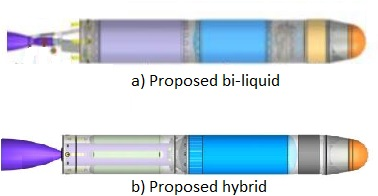
\includegraphics[width=0.5 \textwidth]{figures/heritage/biPropellantSSTOMAV_vaughan2016technology-And-hybridSSTOMAV_karp2016technology.jpg}
%\caption{Current proposed designs. a) is one of the bi-liquid designs proposed by \cite{vaughan2016technology}. b) is the hybrid design proposed by \cite{karp2016technology}. Not to scale.}
%\label{fig:biPropellantSSTOMAV_vaughan2016technology-And-hybridSSTOMAV_karp2016technology}
%\end{figure}


\noindent
Unfortunately, not much has been published on the specific flight parameters, such as drag coefficient and reference area, of these new designs. Fortunately, the size requirements of the \ac{MAV} have not changed (much) between the 2012 studies and the current designs. Therefore these parameters can be approximated by looking at some of the previous baseline designs such as the two-stage liquid-propellant rocket shown in \Cref{fig:baseline_liquid2_trinidad2012}. 


\begin{figure}[H]
\centering
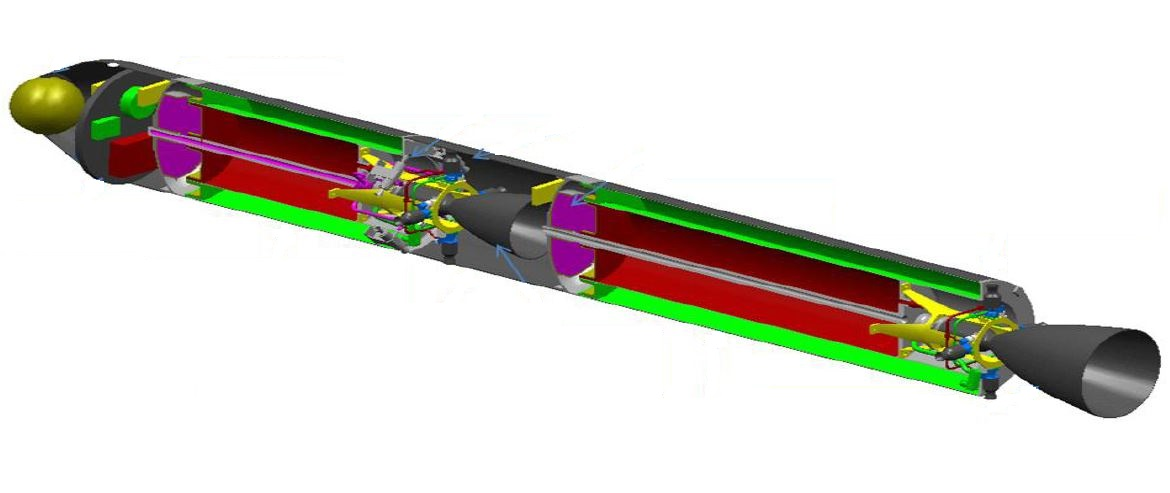
\includegraphics[width=0.5 \textwidth]{figures/launcher_methods/baseline_liquid2_trinidad2012.jpg}
\caption{Baseline design by \cite{trinidad2012} on which the \ac{MAV} design used in this research is mainly based.}
\label{fig:baseline_liquid2_trinidad2012}
\end{figure}

\noindent
This concept by \cite{trinidad2012} had a diameter of approximately 340 mm, resulting in an approximate cross-sectional area of 0.091 m$^{2}$. Unfortunately, the paper does not mention anything about the drag coefficient. However, \cite{whitehead2004mars} provided a general drag coefficient graph as a function of the Mach number for a generalized shape very similar to most \ac{MAV} concepts. Therefore, this simplified relation, shown in \Cref{fig:dragcoeff_whitehead2004mars} is used in this thesis research as well.

\begin{figure}[H]
\centering
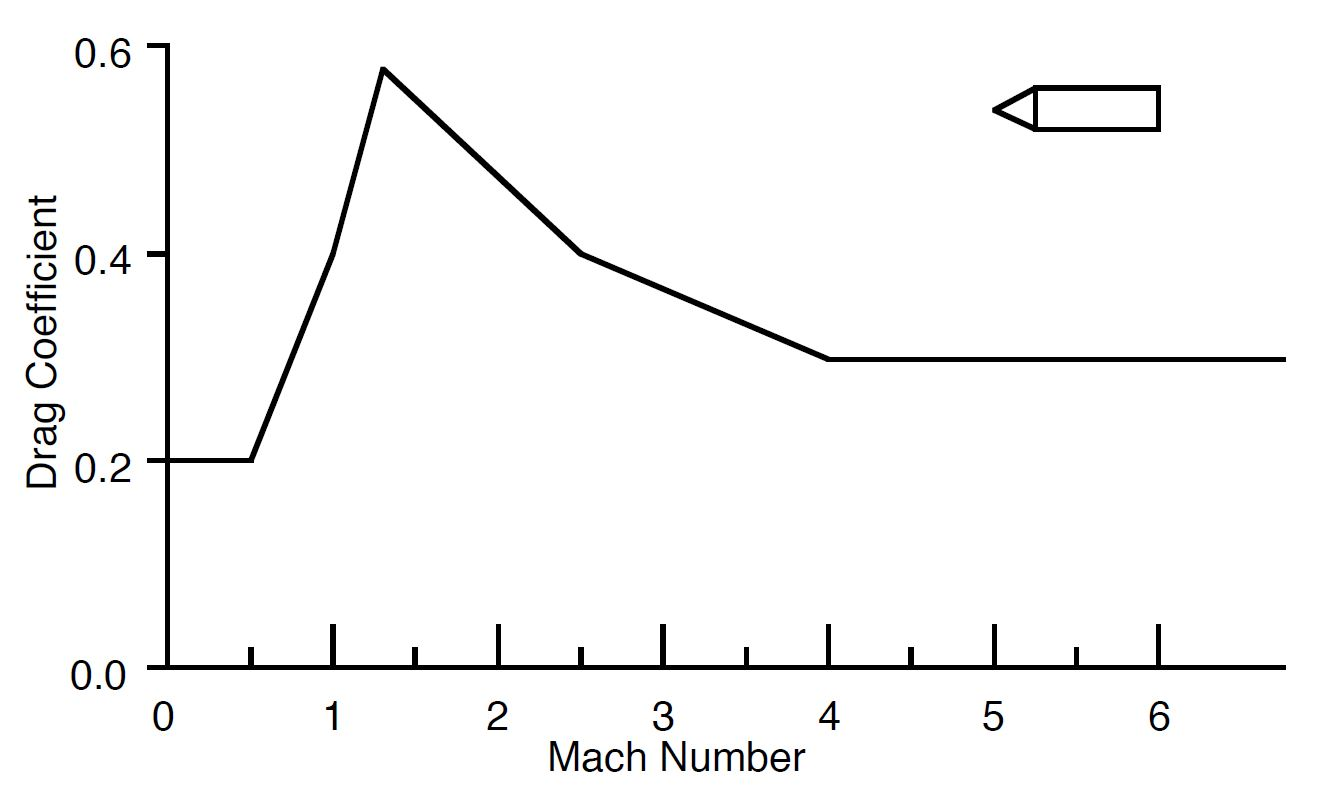
\includegraphics[width=0.5\textwidth]{figures/launcher_methods/dragcoeff_whitehead2004mars.jpg}
\caption{Drag coefficient as a function of Mach number \citep{whitehead2004mars}}
\label{fig:dragcoeff_whitehead2004mars}
\end{figure}

\noindent
These two parameters are crucial in determining the drag force acting on the \ac{MAV} during the ascent. This drag force acts on the \ac{MAV} in what is called the aerodynamic frame. In this research it is assumed that both the angle of attack and the side-slip angle are zero, such that the aerodynamic frame and the body frame coincide.

One of the problems with trajectories is that different perturbations act differently on the vehicle and are easier to express in different reference frames using different formulations. In the end, however, the state will have to be expressed in one reference frame, which means that the drag force will have to be transformed to another frame. More information on these different frames is provided in \Cref{sec:stateAndStateDerivatives}.


%\section{Mars 2020 landing site}
%\label{sec:mars2020LandingSite}
%Show the potential landing sites and the reference site.


%\section{Reference Frames}
%\label{sec:referenceSystems}
%In this research problem, different perturbations are best modelled in different reference frames. One example is the drag acceleration acting in the aerodynamic frame. However, the integration will be performed in the inertial frame. A collection of all the different frames required is shown in \Cref{fig:allFiveReferenceFrames_mooij2013fd-trinidad2012-mooij1994motion}.
%
%\begin{figure}[H]
%\centering
%\subfloat[]{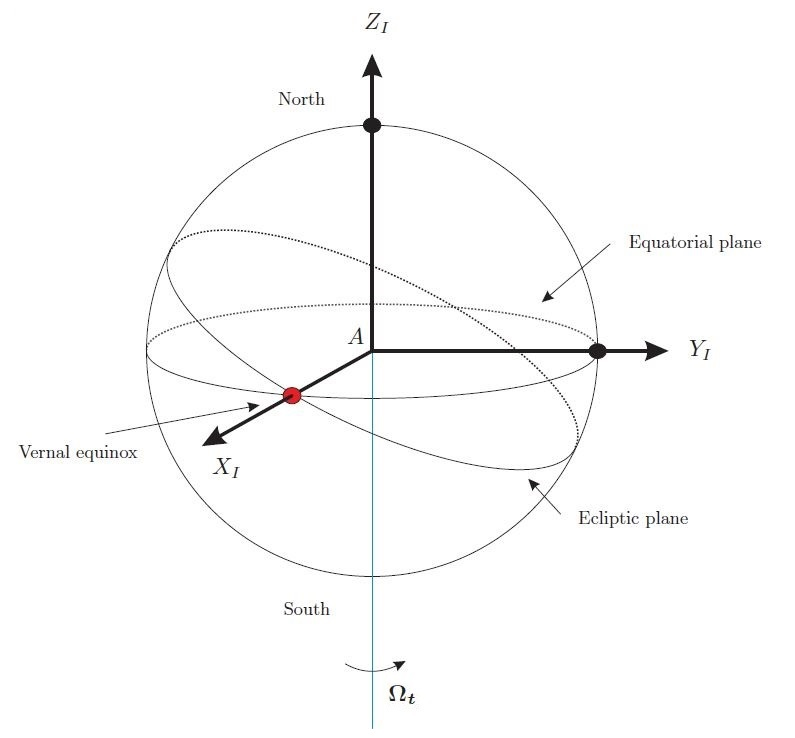
\includegraphics[width=0.5\textwidth]{figures/reference_frames/eci_mooij2013fd_noBox.jpg}\label{subfig:eci_mooij2013fd_noBox}} 
%\subfloat[]{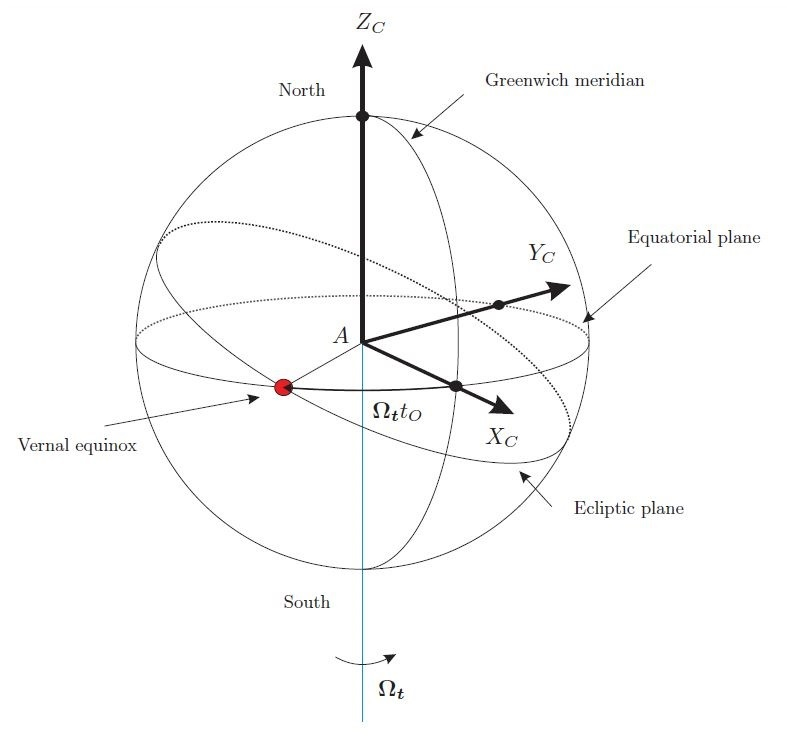
\includegraphics[width=0.5\textwidth]{figures/reference_frames/ecef_mooij2013fd_noBox.jpg} \label{subfig:ecef_mooij2013fd_noBox}}\\
% 
%\subfloat[]{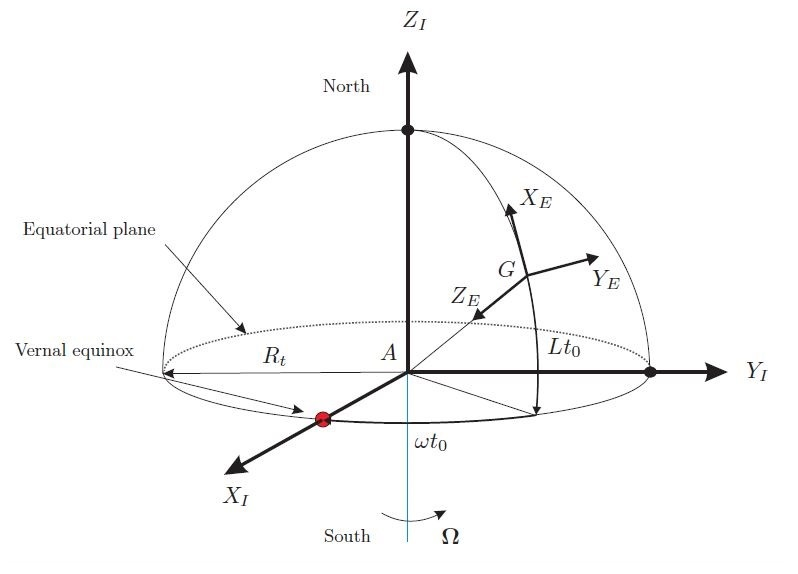
\includegraphics[width=0.5\textwidth]{figures/reference_frames/vcne_mooij2013fd_noBox.jpg}\label{subfig:vcne_mooij2013fd_noBox}} 
%\subfloat[]{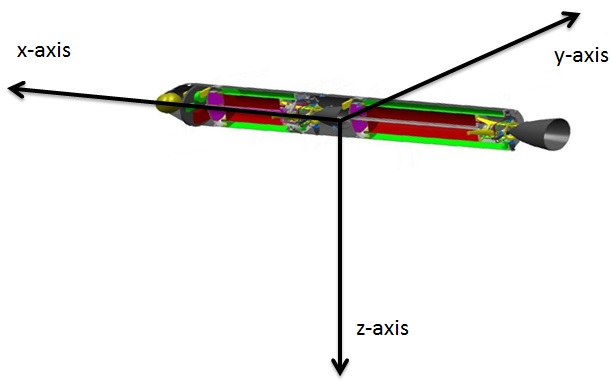
\includegraphics[width=0.5\textwidth]{figures/reference_frames/baseline_liquid_trinidad2012_bframe.jpg}\label{subfig:baseline_liquid_trinidad2012_bframe}}\\
%
%\subfloat[]{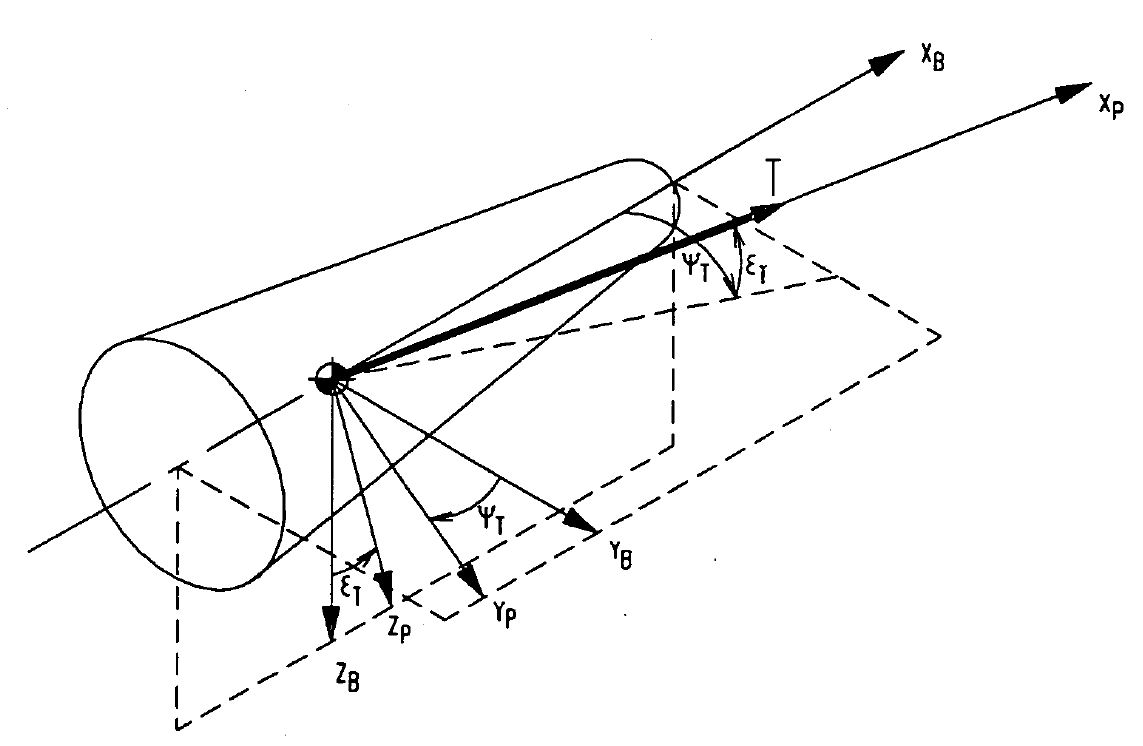
\includegraphics[width=0.5\textwidth]{figures/reference_frames/propframe_mooij1994motion.jpg}\label{subfig:propframe_mooij1994motion}}
%
%
%
%\caption{Used reference frames \protect\subref{subfig:eci_mooij2013fd_noBox} (Mars centred) Inertial frame, \protect\subref{subfig:ecef_mooij2013fd_noBox} (Mars centred) Rotational frame, \protect\subref{subfig:vcne_mooij2013fd_noBox} (Vehicle centred) Vertical frame \citep{mooij2013fd}, \protect\subref{subfig:baseline_liquid_trinidad2012_bframe} (Vehicle centred) Body frame \citep{trinidad2012} and \protect\subref{subfig:propframe_mooij1994motion} (Vehicle centred) Propulsion frame \citep{mooij1994motion}. } 
%\label{fig:allFiveReferenceFrames_mooij2013fd-trinidad2012-mooij1994motion} 
%\end{figure} 
%
%
%%\begin{figure}[H]
%%\centering
%%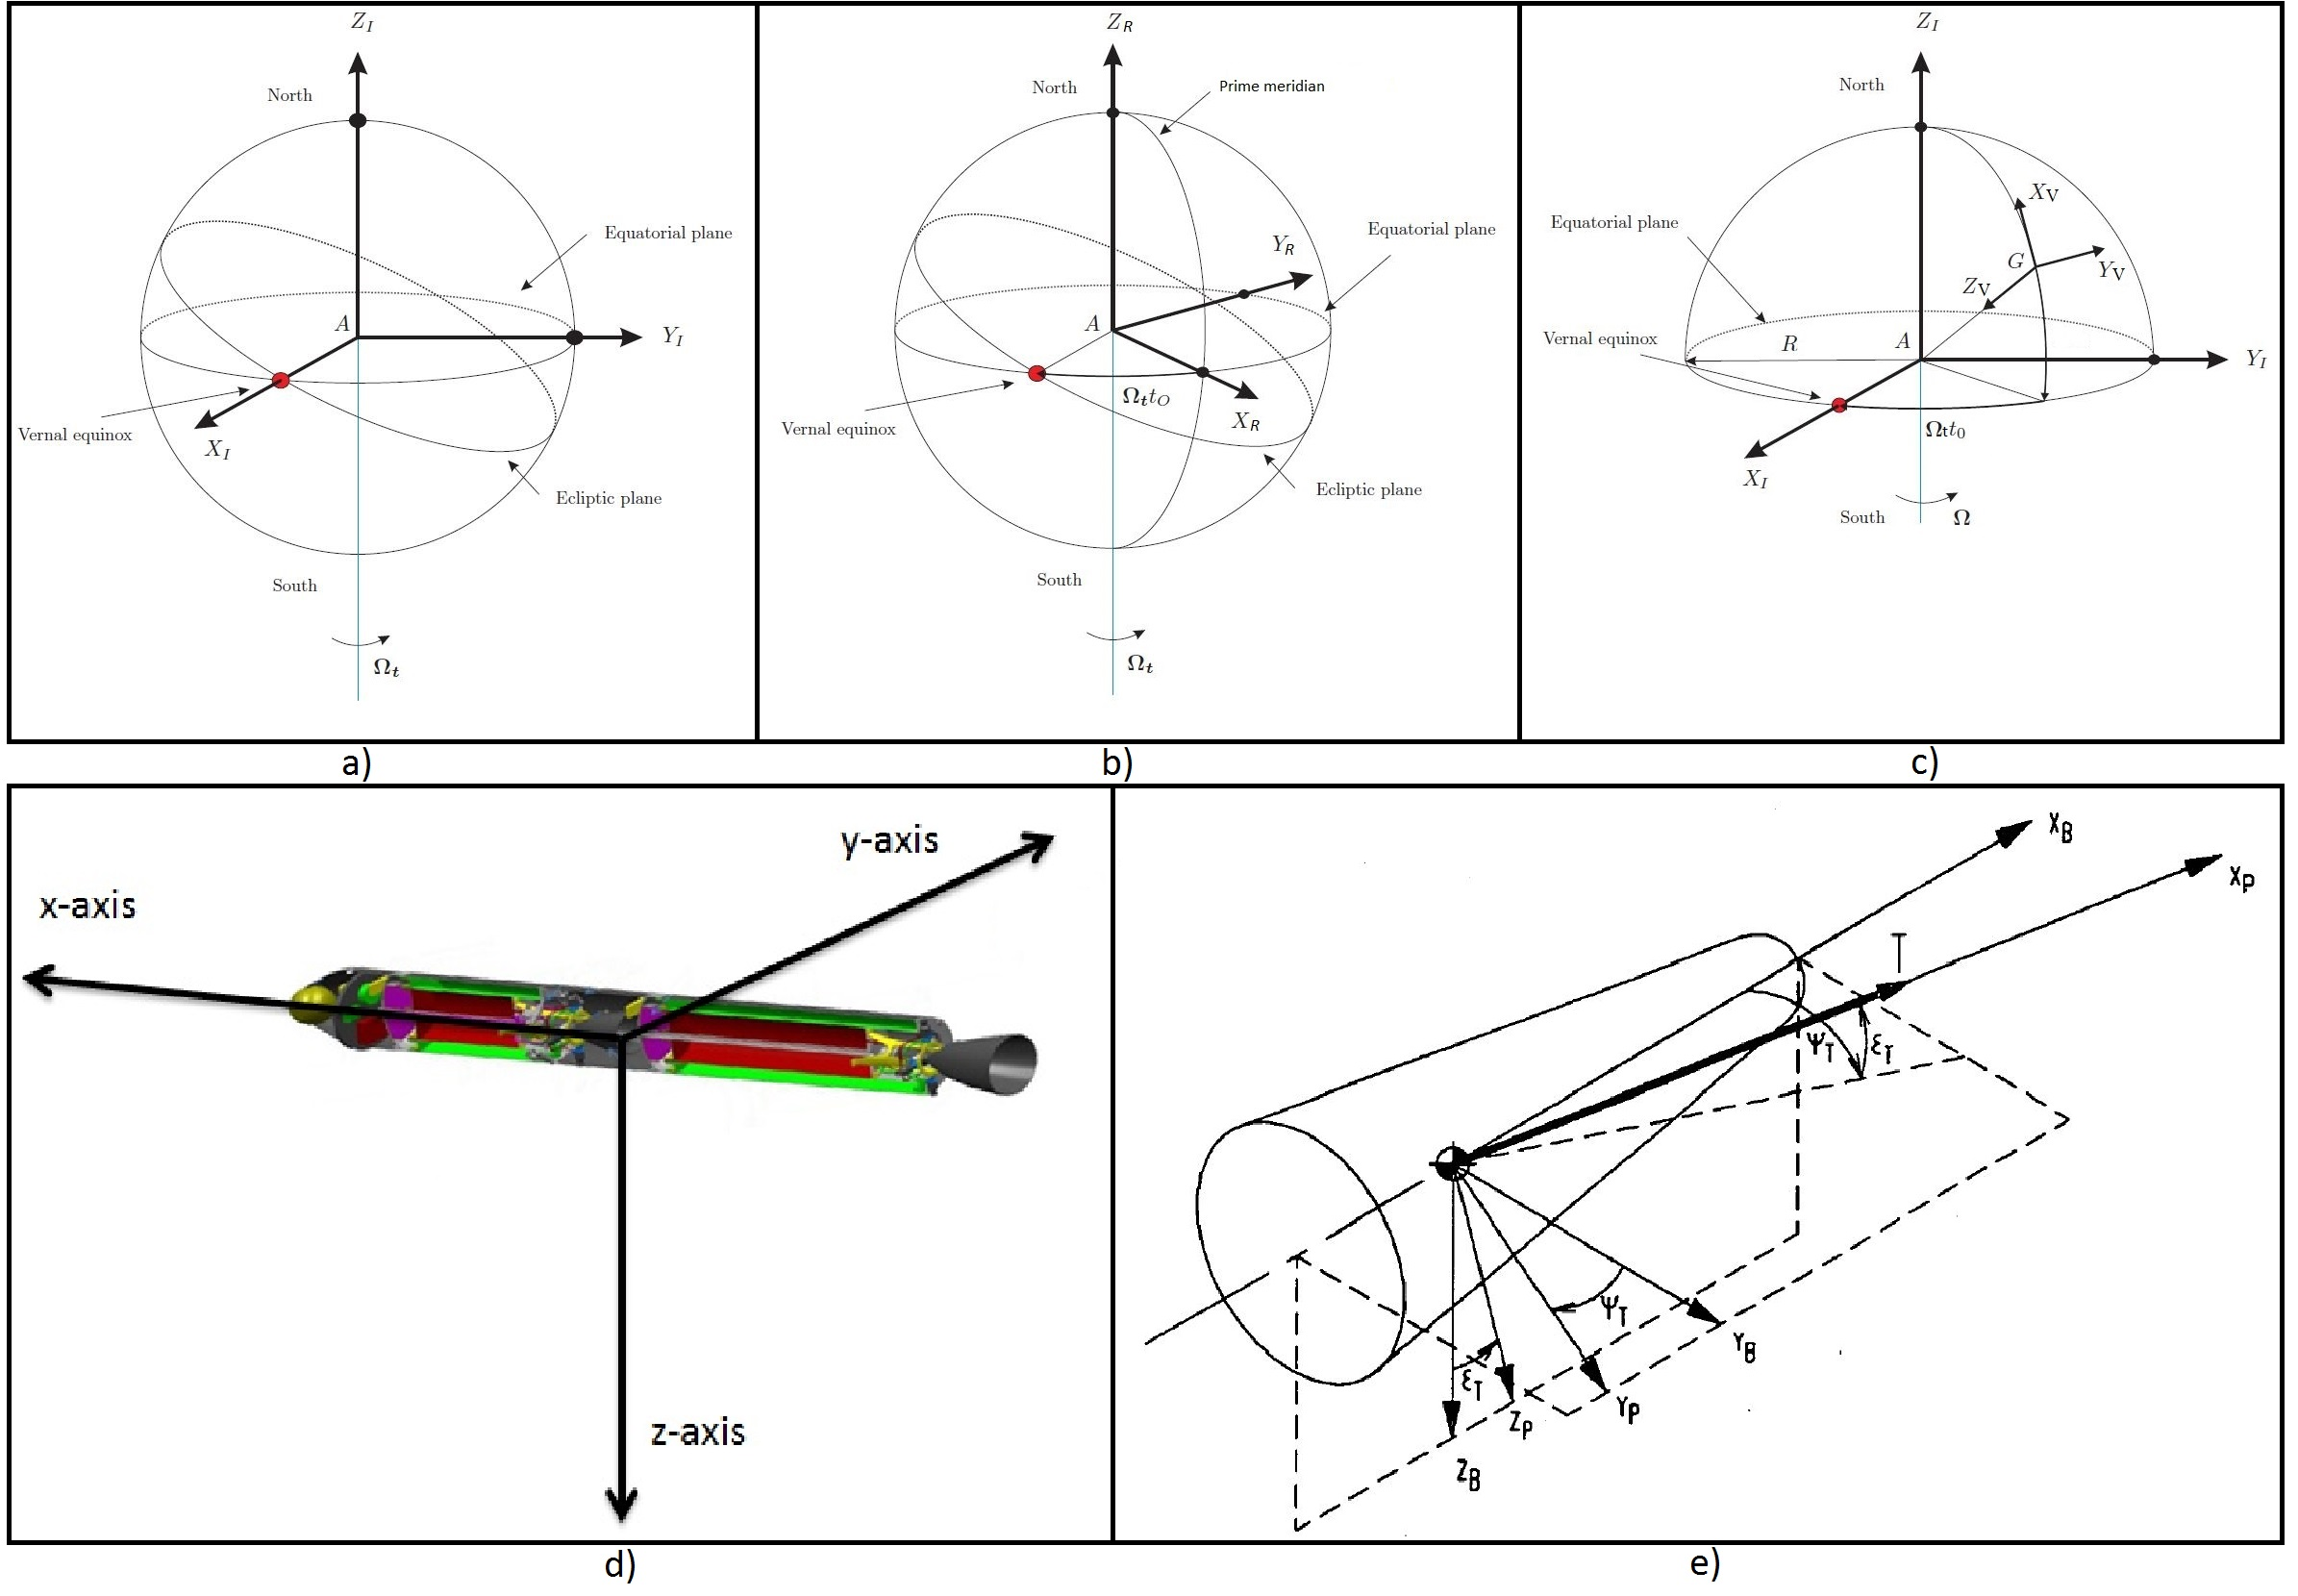
\includegraphics[width=1.0\textwidth]{figures/reference_frames/allFiveReferenceFrames_mooij2013fd-trinidad2012-mooij1994motion.jpg}
%%\caption{a) (Mars centred) Inertial frame, b) (Mars centred) Rotational frame, c) (Vehicle centred) Vertical frame \citep{mooij2013fd}. d) (Vehicle centred) Body frame \citep{trinidad2012}. e) (Vehicle centred) Propulsion frame \citep{mooij1994motion}.}
%%\label{fig:allFiveReferenceFrames_mooij2013fd-trinidad2012-mooij1994motion}
%%\end{figure}
%
%\noindent
%This means that the accelerations have to be translated into the inertial frame through the presented frames. One way to do this is by using so-called transformation matrices ($\mathbb{T}$). These transformation matrices are composed of rotations around different axes over an associated angle $\phi$. An alternative would be to use quaternions instead, which make use of complex numbers. However, due to the workings of \ac{TSI} this was not easily implemented here which is why normal Euler angle transformations were used as the baseline for the rotation equations.  \Cref{fig:exampleXtrans_mooij2013stat} shows a general rotation around the x-axis. When this is set in a matrix, the transformation over the x-, y- and z-axis can be defined in the respective transformation matrices as described by \Cref{eq:allTransMatr}. 
%
%\nomenclature[Rb0]{$\mathbb{T}$}{Transformation matrix \nomunit{-}}
%
%\begin{figure}[!ht]
%\centering
%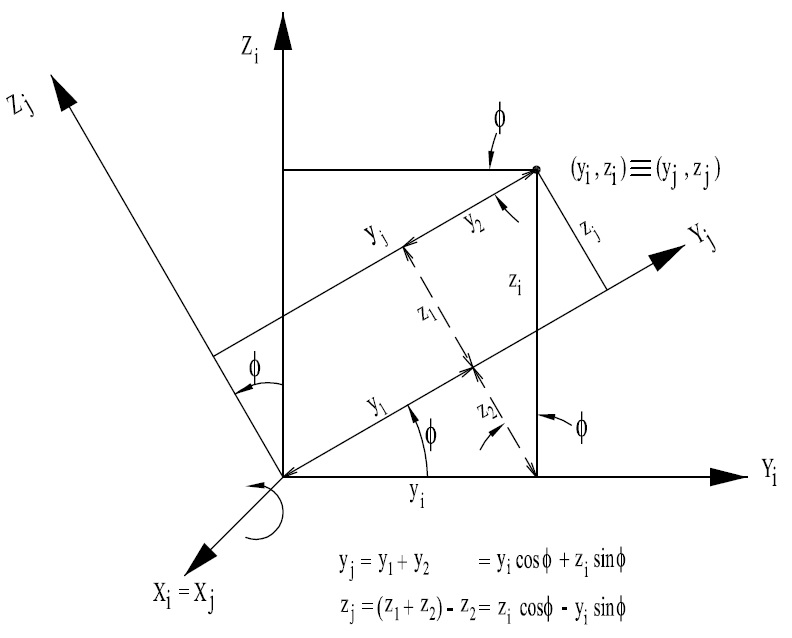
\includegraphics[width=0.5\textwidth]{figures/reference_frames/xtrans_mooij2013stat.jpg}
%\caption{General rotation around the x-axis \citep{mooij2013stat}.}
%\label{fig:exampleXtrans_mooij2013stat}
%\end{figure}
%
%
%\begin{equation} \label{eq:allTransMatr}
%\mathbb{T}_{\mathbf{x}}(\phi)=\begin{bmatrix}
%1 & 0 & 0 \\
%0 & \cos\phi & \sin\phi \\
%0 & -\sin\phi & \cos\phi \\
%\end{bmatrix}, 
%\mathbb{T}_{\mathbf{y}}(\phi)=\begin{bmatrix}
%\cos\phi & 0 & -\sin\phi \\
%0 & 1 & 0\\
%\sin\phi & 0 & \cos\phi \\
%\end{bmatrix}, 
%\mathbb{T}_{\mathbf{z}}(\phi)=\begin{bmatrix}
%\cos\phi & \sin\phi & 0\\
%- \sin\phi & \cos\phi & 0\\
%0 & 0 & 1\\
%\end{bmatrix}
%\end{equation}
%
%\nomenclature[Ga4]{$\phi$}{General Euler angle \nomunit{rad}}
%
%%More information on the different reference frames and the transformation matrices can be found in \Cref{app:appendixAA-referenceSystemTransformations}. \\
%\noindent
%Besides different reference frames, there are also different coordinate systems in which the state of a vehicle can be expressed. Three of the most used coordinate systems in space flight problems are the cartesian, spherical and keplerian system, and all of those systems (or formulations) are used in this research.\\ 
%This also means that the state should be transformed between these different coordinate sets. In \Cref{fig:sphertocart_noomen2013basicFirst} it is shown how the position of a point can be described in either spherical coordinates or cartesian coordinates.
%
%
%\begin{figure}[H]
%\centering
%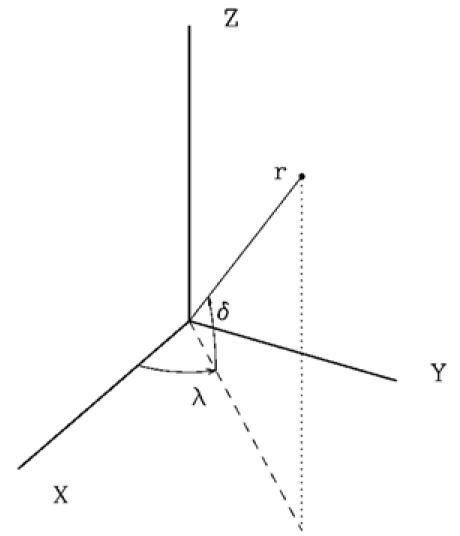
\includegraphics[width=0.3\textwidth]{figures/reference_frames/sphertocart_noomen2013basic.jpg}
%\caption{Position expressed either in the cartesian (x,y,z) or in the spherical system ($r$, $\delta$, $\lambda$) \citep{noomen2013basic}.}
%\label{fig:sphertocart_noomen2013basicFirst}
%\end{figure}
%
%\noindent
%From this figure the relation can be described between the two different systems. This relation is important to allow for the translation between parameters expressed in one system to the other. More information on the transformations and coordinate system relations can be found in \Cref{app:appendixAA-referenceSystemTransformations}.
%%
%%If the cartesian coordinates are known, the spherical coordinates can be computed using \Cref{eq:cart2spher}.
%%
%%\begin{equation} \label{eq:cart2spher}
%%\begin{split}
%%r &= \sqrt{x^{2}+y^{2}+z^{2}}\\
%%\delta &= \arcsin \left(\dfrac{z}{r}\right)\\
%%\lambda &= \arctan \left(\dfrac{y}{x}\right)\\
%%\end{split}
%%\end{equation}
%
%\nomenclature[Rb1]{$x$}{x-position coordinate \nomunit{m}}
%\nomenclature[Rb5]{$y$}{y-position coordinate \nomunit{m}}
%\nomenclature[Rb5]{$z$}{z-position coordinate \nomunit{m}}
%\nomenclature[Ra5]{$r$}{Radius \nomunit{m}}
%\nomenclature[Ga1]{$\delta$}{Latitude \nomunit{rad}}
%\nomenclature[Ga3]{$\lambda$}{Inertial longitude \nomunit{rad}}

%
%
%\noindent
%The same calculation can be done from the spherical system to the Cartesian system. The corresponding equations for that calculation are shown in \Cref{eq:spher2cart}.
%
%\begin{equation} \label{eq:spher2cart}
%\begin{split}
%x &= r\cos\delta\cos\lambda\\
%y &= r\cos\delta\sin\lambda\\
%z &= r\sin\delta\\
%\end{split}
%\end{equation}
%
%%All the coordinate transformations can be found in \Cref{app:appendixAA-referenceSystemTransformations}, which include both position and velocity vectors. 
%\noindent
%These standard transformations are essential in defining the models and setting up the equations of motion.


%Add a section on reference systems (maybe including appendix on the transformations etc.)









